\section{Method}
\label{sec:method}
Bug bounty programs work on the premise that humans as a crowd are efficient at searching and finding bugs. Their mere existence is a {\it de facto} recognition that market approaches for bug discovery bring efficiency, beyond in-house security. Bug bounty programs signal that organizations are ready to complement their vertical cost-effective security operations with market approaches, which are traditionally perceived as less cost-effective, yet more adaptive \cite{coase1937}. Early on, Brady et al. \cite{brady1999murphy} have offered a hint for the existence of such markets for bugs: according to their proposed theory, each researcher has slightly different skills and mindset. When a security researcher tests a software piece by choosing the inputs, she offers a unique operational environment. This environment is prone to the discovery of new bugs, which may not have been seen by other researchers. The proposed theory by Brady et al. \cite{brady1999murphy} intrinsically justifies the existence of bug bounty program structures as markets, which provide the necessary diversity to account for the highly uncertain risk horizon of bug discovery. Here, we develop a quantitative method to formalize a mechanism and to test the theory proposed in \cite{brady1999murphy}. This validation step shall help provide organizational design insights for bug bounty programs.\\

For that, we investigate the interplay between the vulnerability discovery process and the cumulative rewards distributed to security researchers within and across 35 public bounty programs hosted on HackerOne. When a bug bounty program starts, it attracts a number of security researchers, who in turn submit bug reports. Subsequent bug discoveries get increasingly difficult for each individual researcher, and to some extent for all researchers together. The difficulties faced by security researchers can be technical. They can also be the result of insufficient or conflicting incentives. Here, we develop and test a model, which accounts for both technical difficulties and insufficient incentives. We further address conflicting incentives by measuring the effect of newly launched bug bounty programs on incumbent programs.\\

Starting from an initial probability of discovering the first vulnerability $P(k=0) = 1$, the probability to find a second bug is a fraction of the former probability: $P_{k+1} = \beta \cdot P_k$ with $\beta$ a constant strictly smaller than one. The probability that no more discoveries will be made after $k$ steps is given by $P_k = \beta^{k} (1-\beta)$. Conversely, starting from the initial reward $R_0 = R(k=0)$, the subsequent reward $R_1 = \Lambda_1 \cdot R_0$, and further additional reward $ R_2 = \Lambda_2 \Lambda_1 \cdot R_{0}$. After $n$ steps, the total reward is the sum of all past rewards: 

\begin{equation}
R_{n} = R_{0} \sum_{k=1}^{n} \Lambda_1 ... \Lambda_k.
\end{equation}

Thus, $R_{n}$ is the recurrence solution of the  
Kesten map ($R_{n} = \Lambda_n R_{n-1} +R_0$)
\cite{kesten1973random,sornette1997convergent}:  as soon as amplification occurs (technically, 
some of the factors $\Lambda_k$ are larger than $1$), the distribution
of rewards is a power law, whose exponent $\mu$ is a function of $\beta$
and of the distribution of the factors $\Lambda_k$. In the case where
all factors are equal to $\Lambda$, this model predicts three possible regimes for the distribution of rewards (for a given program): thinner than exponential for $\Lambda < 1$, exponential for $\Lambda = 1$, and power law for $\Lambda > 1$ with exponent $\mu = |\ln \beta|/ \ln \Lambda$ \cite{sornette2013exploring}. The expected payoff of vulnerability discovery is given by,

\begin{equation}
\label{ }
U_k = P_k \times R_k,
\end{equation}

\noindent with both $P_k$ and $R_k$ random variables respectively determined by $\beta$ and $\Lambda$. Because $U_k$ is a multiplication of diverging probability and reward components, its nature is reminiscent of the St. Petersburg paradox (or St. Petersburg lottery), proposed first by the Swiss Mathematician Nicolas Bernoulli in 1713, and later formalized by his brother Daniel in 1738 \cite{bernoulli1954exposition}. The St. Petersburg paradox states the problem of decision-making when both the probability and the reward are diverging for $k \rightarrow \infty$: a player has a chance to toss a fair coin at each stage of the game. The pot starts at two and is doubled every time a head appears. The first time a tail appears, the game ends and the player wins whatever is in the pot. Thus, the player wins two if a tail appears on the first toss, four if a head appears on the first toss and a tail on the second, eight if a head appears on the first two tosses and a tail on the third, and so on. The main interest of Bernoulli was to determine how much a player would be ready to pay for this game, and he found that very few people would like to play this game even though the expected utility increases (in the simplest case proposed by Bernoulli, $U_n = \sum_{k=0}^{n} U_k = n$) \cite{bernoulli1954exposition}. The situation of a security researcher differs from the St. Petersburg lottery as bug search costs are incurred at every step. Since these costs influence the probability to find an additional bug, they can be at least partially integrated in $P_k$. We could assume equivalently that costs are integrated into a net utility as $U^{*}_k = U_k - c_k$. Here, we do not factor these costs in because their exact nature is largely undetermined and our data do not offer a reliable proxy. The security researcher may also decide to stop searching for bugs in a program, at any time $k$: this is equivalent to setting $P_{k+1} = 0$.\\

The expected payoff $U_k$ therefore determines the incentive structure for security researchers, given that the bounty program manager can tune $R_0$ and to some extent $\Lambda$. The utility function may also incorporate non-monetary incentives, such as reputation: finding a long series of bugs may signal some fitness for a bug bounty program and thus create a permanent job opportunity \cite{moussouris2016}. Similarly, discovery of a rare (resp. critical) bug that no other researcher has found before has a strong signaling effect, which can help make a career. However, these strategies are high-risk high-return. Therefore, they result in additional fame. In the next section, we will calibrate our model to the bug discovery process associated with 35 bounty programs publicly documented on the HackerOne platform.

 %However, rules are generally set upfront and shall not be changed in the course of the bounty program. Changing game rules is risky as it may undermine trust in the program. Here, we assume that bounty program managers don't tune their reward policy after the bug bounty program has started. 

%\sout{In principle, the manager could set $R_0$ to influence $P_0$ and indirectly $P_{k}$. Mapping the discovery rank $k$ into the rate of discovery may also help considering discounting aspects in presence of competing opportunities and inter-temporal choices under uncertainty \cite{loewenstein1992anomalies}. A new public bounty program is launched at a Poisson rate, approximately every 2 months, and each launch brings its windfall effect, leaving the researcher with the choice to either keep digging increasingly harder vulnerabilities (rare but with higher reward), or turning to the low hanging fruit (frequent but with low reward) of a new program. We shall therefore verify whether newly launched programs actually influence security researchers.}


%The propensity for security researchers to keep searching for vulnerabilities is conditioned by the trend of $U(k)$: if $U \rightarrow 0$ when $k \rightarrow \infty$, then it's likely that they will leave the program (it's a bit sketchy here). If do not consider the costs (i.e., effort spent on finding the $k^{th}$ bug, which we cannot measure here (see next subsection on timing effects), but which is indirectly captured by $P(k)$), then in the presence of a variety of programs at different stages of their life (i.e., at different values of $k$), the security researcher is left with comparing utility between programs.

%\begin{figure}
%\begin{center}
%%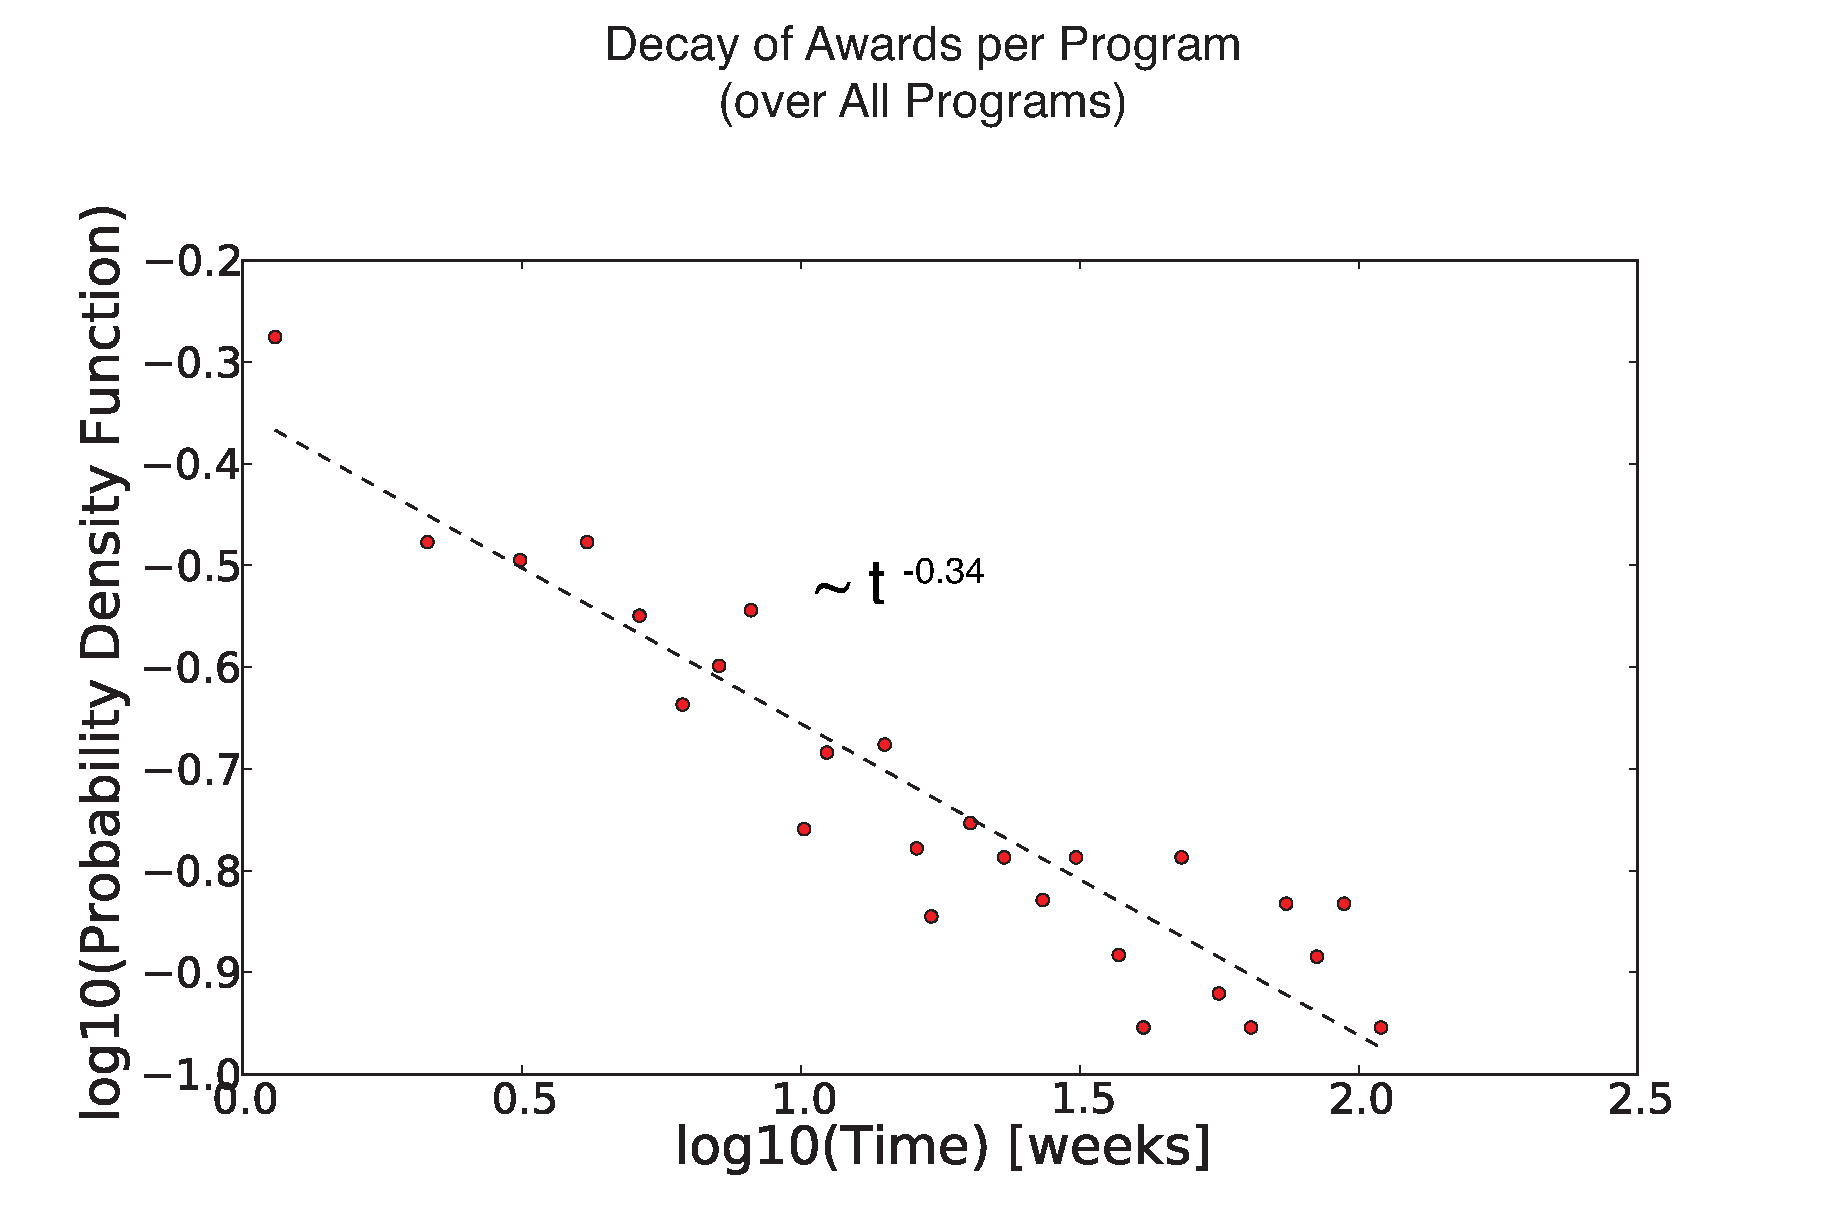
\includegraphics[width=10cm]{figures/decay.eps}
%\caption{Distribution of discovery waiting time between ranks $\rightarrow$ the hope is to find that time increases as $k \rightarrow \infty$.}
%\label{fig:decay}
%\end{center}
%\end{figure}



%The incentive mechanism is then completely driven by the probability of discovery of the $k+1$ vulnerability given that $k$ bugs have already been discovered on the one hand, and by the expected reward for the $k+1$ discovery on the other hand. When the probability of finding a bug decreases fast while the reward for a new bug increases fast, in such a way that the product $f_k \times R_k$ remains constant, then the expected value of the game increases linearly as $k \rightarrow \infty$. This problem is reminiscent 


%When a bug bounty program (by an organization) is launched immediate vulnerabilities are found by security researchers and rewarded by organizations. The cost of finding a new vulnerability increases as more discoveries occur, and thus, incentives should be set accordingly to keep onboard security researchers, or at least, the best researchers who have the capabilities to find increasingly subtle problems. 



%Searching for bugs in software is an attrition process: When the search starts, obvious bugs are found first. Subsequent bug discoveries get increasingly difficult. When a bug bounty program (by an organization) is launched immediate vulnerabilities are found by security researchers and rewarded by organizations. The cost of finding a new vulnerability increases as more discoveries occur, and thus, incentives should be set accordingly to keep onboard security researchers, or at least, the best researchers who have the capabilities to find increasingly subtle problems. 
%
%{\bf aim 1:} understand the evolution of expected utility of security researchers as an increasing amount of vulnerabilities get discovered for a given program. And how the incentive mechanism varies from one program to another\\
%
%{\bf aim 2:} understand how bug bounties compete with each others? Each time, a new bug bounty program is launched, a new set of opportunities arises, and security researchers must make a choice (though not a binary choice) between digging further in an existing program (with lower probability to find a vulnerability, but presumably with higher utility) or turning to a new program (with higher probability to find a vulnerability, but presumably with lower utility).
%
%{\bf aim3: } What can we say about the whole eco-system?


